\chapter{Introducci\'on}
\label{cap:intro}

\section{Antecedentes y motivaci\'on}
\label{intro:motivacion}

Para un ser humano el proceso de visión resulta un ejercicio bastante simple, es capaz de distinguir, por ejemplo, cuantas personas hay en una imagen sin esforzarse demasiado aún en condiciones desfavorables por ejemplo, una imagen borrosa o con poca luz, sin embargo, utilizar un computador para realizar dicho ejercicio se torna una tarea desafiante, el área de estudio enfocada en la resolución de este tipo de desafíos es la visión por computador la cual es un campo de estudio dentro de la inteligencia artificial enfocado al modelamiento matemático de los procesos de percepción visual de los seres vivos.

En la actualidad un problema importante de la visión por computador es la detección de personas, esta importancia yace en sus variadas aplicaciones que van desde el entretenimiento en redes sociales, hasta sofisticados sistemas de seguridad en calles o a bordo de automóviles entre otras. En particular la detección de peatones tiene importancia fundamental dentro del contexto de la video vigilancia y para la resolución de este problema se han propuesto variados enfoques, algunos de los más relevantes son la detección holística \citep{dalal2006}, la detección basada en partes \citep{nevatia2005}, o una mezcla de estos enfoques \citep{leibe2005,yu2011}, es conocido el problema de determinar la existencia de un peatón en una determinada ventana de clasificación se encuentra bien estudiado, sin embargo existen aun subproblemas por estudiar y dentro de ellos el estudio de comportamiento de los clasificadores cuando la ventana de clasificación encuentran en la cercanía del ground truth.

\section{Descripci\'on del problema}
\label{intro:problema}

Determinar la existencia de un peat\'on en una secci\'on de una imagen es un problema muy estudiado, sin embargo, dentro de la detección de peatones (d\'onde est\'an los peatones en una imagen) se encuentra el sub-problema del comportamiento del clasificador en el momento de encontrarse evaluando la vecindad cercana al peat\'on.
Un clasificador humano evalúa la presencia de un peat\'on en la imagen analizando la informaci\'on tomada de una ventana o cuadro que se desliza por la imagen y entrega como resultado la determinaci\'on de la existencia de un peatón o no adem\'as de un valor para el nivel de confianza con el cual el clasificador asegura que se trata de un peat\'on.
En forma ideal, la confianza de la respuesta del clasificador s\'olo debe ser muy alta cuando la ventana evaluada se encuentra frente a frente al peat\'on, y no cuando se encuentra en su cercanía. En este \'ultimo caso, la confianza de su respuesta debe ser muy baja. En la figura  a la izquierda se observa en color verde el desplazamiento de la ventana de clasificación y en color rojo el momento en que la venta se encuentra completamente frente al peatón, a la derecha se muestra el resultado si se tratase de un buen clasificador; en un escenario ideal el resultado obtenido debería ser asemejar a la función impulso.

%\ref{fig:xml}

% Figura: \'Arbol XML 1
%\begin{figure}[tp]
%  \centering
%  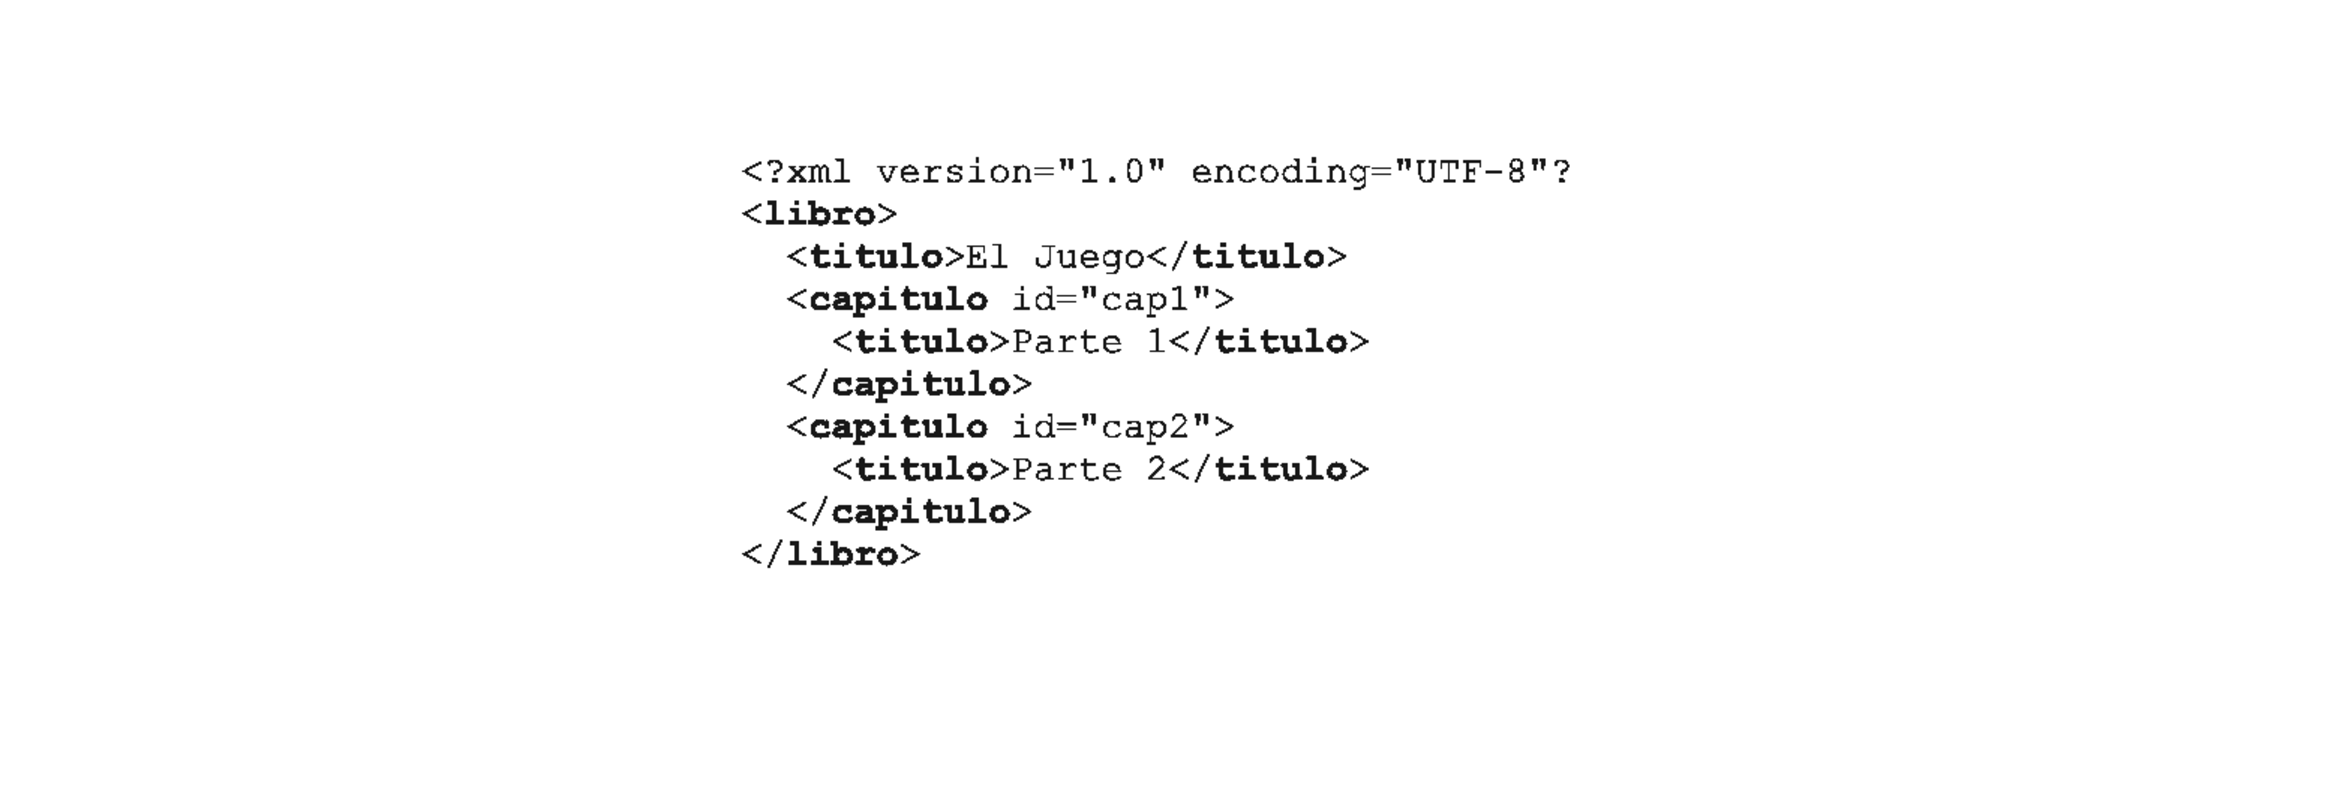
\includegraphics[scale=.5]{images/XML-document-example1}
%  \caption{\em Ejemplo de comportamiento de un clasificador en la vecindad de un peat\'on.}
%  \label{fig:xml}
%\end{figure}


\section{Soluci\'on propuesta}
\label{intro:solucion}

Para so

\section{Objetivos y alcance del proyecto}
\label{intro:objetivos}

\subsection{Objetivo general}

Desarrollar una metodología que permita la comparación y un software de pruebas que permita evaluación sistemática de múltiples clasificadores con el fin de encontrar aquel con mejor sensibilidad espacial para minimizar detecciones múltiples en la vecindad del peatón utilizando el set de datos INRIA

\subsection{Objetivos espec\'ificos}

Para la consecución del objetivo general, se plantean las siguientes metas intermedias:

\begin{enumerate}
  \item Crear un modelo matemático que permita generar un indicador que describa la sensibilidad espacial según la respuesta de los clasificadores.
\item Desarrollar una metodología de evaluación que permita a través de la utilización del indicador comparar la sensibilidad de un clasificador en la vecindad de un peatón.
\item Desarrollar un software modular que permita la automatización de la metodología y la comparación de clasificadores.
\item Implementar los descriptores y clasificadores que no se encuentren previamente implementados para su evaluación.
\item Determinar cuál de los clasificadores corresponde al que posee la mejor sensibilidad espacial para minimizar detecciones múltiples de peatones en el set de datos INRIA
.
\end{enumerate}

\subsection{Alcances}


\section{Metodolog\'ia y herramientas utilizadas}
\label{intro:metodologia}

\subsection{Metodolog\'ia}


\subsection{Herramientas de desarrollo}


\section{Resultados Obtenidos}|
\label{intro:resultados}


\section{Organizaci\'on del documento}
\label{intro:organizacion}

El presente trabajo está dividido en ocho capítulos considerando éste como el primero. En el Capítulo~\ref{cap:preliminares} se 
